\documentclass[12pt]{ucthesis}

\usepackage{etex}
\usepackage[morefloats=125]{morefloats}
\usepackage[hyphens]{url}
\usepackage[caption=false]{subfig}
\usepackage{graphicx}
\usepackage{tabularx}
\usepackage{amssymb}
\usepackage{amsmath}
\usepackage[letterpaper]{geometry}
\usepackage[overload]{textcase}
%\usepackage{color}
\usepackage{xcolor}
\usepackage[nonumberlist,toc]{glossaries}
\usepackage{wrapfig}
\usepackage{longtable}
\usepackage{morefloats}
\usepackage{float}
\usepackage{listings}
\usepackage{makecell}
\usepackage{appendix}
\usepackage[]{algorithm2e}
\usepackage{titlesec}
\usepackage[breaklinks=true,hidelinks,pdfusetitle]{hyperref}
\usepackage{cleveref}
\usepackage{ifthen}

\setcounter{secnumdepth}{3}
\setcounter{tocdepth}{3}

% Added to avoid windows and orphans
\usepackage[all]{nowidow}
% Added to fix spacing between footnote entries
\usepackage{setspace}
\newlength{\myfootnotesep}
\setlength{\myfootnotesep}{\baselineskip}
\addtolength{\myfootnotesep}{-\footnotesep}
\setlength{\footnotesep}{\myfootnotesep} % set spacing between footnotes

\makeindex
\makeglossaries

% Shrink the size of headers
\titleformat{\chapter}[display]
        {\normalfont\normalsize\centering}
        {\ifthenelse{\equal{\thechapter}{A}}{APPENDICES\\[4.3ex]}{}\chaptertitlename\ \thechapter}
        {0pt}{\normalsize\uppercase}
\titlespacing*{\chapter}{0pt}{-20pt}{4.3ex plus .2ex}


\titleformat*{\section}{\normalsize\bfseries}
\titleformat*{\subsection}{\small\bfseries}
\titleformat*{\subsubsection}{\small\bfseries}
\titleformat*{\paragraph}{\small\bfseries}
\titleformat*{\subparagraph}{\small\bfseries}

\bibliographystyle{abbrv}

% Make \tindent indent pages if you have no paragraph indent
\newlength\tindent
\setlength{\tindent}{\parindent}
\setlength{\parindent}{0.in} \setlength{\parskip}{1.em}
\renewcommand{\indent}{\hspace*{\tindent}}
% Otherwise, comment out the above and uncomment this for default indentation on each paragraph
%\setlength{\parindent}{0.25in} \setlength{\parskip}{6pt}

\geometry{verbose,nohead,tmargin=1in,bmargin=1in,lmargin=1.5in,rmargin=1in}

% Different font in captions (single-spaced, bold) ------------
\newcommand{\captionfonts}{\small\bf\ssp}

\newcommand{\mycaption}[2]{\caption[#1 --- #2]{#1 --- #2}}

\makeatletter  % Allow the use of @ in command names
\long\def\@makecaption#1#2{%
  \vskip\abovecaptionskip
  \sbox\@tempboxa{{\captionfonts #1: #2}}%
  \ifdim \wd\@tempboxa >\hsize
    {\captionfonts #1: #2\par}
  \else
    \hbox to\hsize{\hfil\box\@tempboxa\hfil}%
  \fi
  \vskip\belowcaptionskip}
\makeatother   % Cancel the effect of \makeatletter
% ---------------------------------------

% Define Appendix refs
\crefname{app}{appendix}{appendices}
\Crefname{app}{Appendix}{Appendices}

% Add Figures folder to the graphics path
\graphicspath{{Figures/}{figures/}}

% Options for hyperref
\hypersetup{
    bookmarksnumbered=true,
    bookmarksopen=false,
    bookmarksopenlevel=0,
    colorlinks=false,
    pdfstartview=Fit,
    pdfborder={0 0 0},
}

\newcounter{qcounter}
\providecommand{\keywords}[1]{\textbf{\textit{Keywords:}} #1}


\newcommand{\titletext}{Clustering Web Users By Mouse Movement to Detect Bots and Botnet Attacks}


\begin{document}

% Declarations for Front Matter
\title{Your Thesis Title}
\author{Your Name}
\degreemonth{June} \degreeyear{2014} \degree{Master of Science}
\defensemonth{June} \defenseyear{2014}
\numberofmembers{2}
   \chair{Alexander Dekhtyar, Ph.D. \linebreak Professor of Computer Science}
   \othermemberA{Aaron Keen, Ph.D. \linebreak Professor of Computer Science}
   \othermemberB{Franz Kurfess, Ph.D. \linebreak Professor of Computer Science}
\field{Computer Science} \campus{San Luis Obispo}
\copyrightyears{seven}


\maketitle

\begin{frontmatter}

\title{\titletext{}}

% Custom made for Cal Poly (by Mark Barry, modified by Andrew Tsui).
\copyrightpage

% Custom made for Cal Poly (by Andrew Tsui).
\committeemembershippage

\begin{abstract}
The need for website administrators to efficiently and accurately detect the presence of web bots has shown to be a challenging problem.
As the sophistication of modern web bots increases, specifically their ability to more closely mimic the behavior of humans, web bot detection schemes are more quickly becoming obsolete by failing to maintain effectiveness~\cite{10.1109/DSN.2013.6575366}~\cite{ROVETTA2020102577}~\cite{STEVANOVIC2013698}.
Though machine learning-based detection schemes have been a successful approach to recent implementations, web bots are able to apply similar machine learning tactics to mimic human users, thus bypassing such detection schemes.
This work seeks to address the issue of machine learning-based bots bypassing machine learning-based detection schemes, by introducing a novel unsupervised learning approach to cluster users based on behavioral biometrics.
The idea is that, by differentiating users based on their behavior~\cite{FEHER201219}, for example how they use the mouse or type on the keyboard, information can be provided for website administrators to make more informed decisions on declaring if a user is a human or a bot.
This approach is similar to how modern websites require users to login before browsing their website; which in doing so, website administrators can make informed decisions on declaring if a user is a human or a bot.
An added benefit of this approach is that it is a human observational proof (HOP); meaning that it will not inconvenience the user (user friction) with human interactive proofs (HIP) such as CAPTCHA, or with login requirements.
\end{abstract}

\begin{acknowledgements}
\noindent
Thanks to:
\begin{itemize}
    \item Dr. Franz Kurfess, for your never-ending support and understanding
    \item Dr. Phoenix Fang and Dr. Maria Pantoja, for your advice and suggestions as committee members
    \item My family, for supporting and motivating me
    \item Dr. John Walker, for your statistical advice
    \item Dr. Alex Dekhtyar, for your advice on machine learning strategies
    \item Dr. Theresa Migler, Kurt Voelker, and Kurt Mammen, for recommending my admission into this grad program
    \item Dr. Chris Lupo, for never being too busy to meet with a student and, for giving me a lecturing opportunity
    \item Leanne Fiorentino, for always making it happen
    \item Skyler Ceronio, for being a solid dude
    \item Nate Jones, for giving me a career-starting internship opportunity
    \item Andrew Guenther, for uploading this template
\end{itemize}

\end{acknowledgements}

\tableofcontents

\listoftables

\listoffigures

% Add CHAPTER into table of contents.
\addtocontents{toc}{%
   \noindent CHAPTER
}

\end{frontmatter}

\pagestyle{plain}

\renewcommand{\baselinestretch}{1.66}



\chapter{Introduction}
A web bots is a programmatic simulation of a human user web browsing session. Similarly, a botnet is a collection of web bots working in unison. Most of these bots are programmed with the intention of foregoing remedial and repetitive tasks that a human user would be required to do. Some examples of these tasks may include searching for specific items, of a given criteria, through a large number of items on an ecommerce site like Amazon. Another example can be the action of downloading lists textual data on a web page that would require the user to manually save. There are many use cases for these programmatic simulations, otherwise known as web bots. Unfortunately, web bots are often used maliciously or irresponsibly, thus introducing a number of problems for the users and administrators of a web site~\cite{1ee426975c3d46d2ba6ef5c2d76384c5}. Efforts to detect these web bots have proven to be successful in many cases. However, due to the increasing sophistication of web bots, said detection schemes are continuously bypassed and deemed obsolete. This work addresses some of these issues.


\chapter{Related Work}\label{ch:related-work}
The unsupervised machine learning approach of this thesis research was inspired by a few preexisting implementations of the like.
By observing the strengths and weaknesses of these implementations, the outcome of this work is expected to be an improvement and beneficial contribution to the field of web bot and botnet detection research.
This section will provide a synopsis and evaluation of the related work that provided inspiration to this work.


\section{Supervised Learning}\label{sec:supervised-learning}
There are several supervised learning~\ref{subsec:supervised-and-unsupervised-learning-methods} bot detection schemes that utilize labeled datasets to train models in their implementation.

\subsection{Deep Learning with Mouse Behavior Metrics}\label{subsec:deep-learning-with-mouse-behavior}
The detection scheme described in~\cite{deep_learning_detection_with_mouse_behavior} analyzes the mouse movement and operations of a user to decide whether these gestures are consistent with that of a human user or bot user.
Images containing the spatial and kinetic information that represents the mouse behavioral metrics are passed into a deep neural network for making the bot or not decision.
Representing the models in such a way has enabled the use of a Convolutional Neural Network, or "CNN", to automate feature learning from a user's raw mouse position data.

Rather than following the patterns of previous implementations that fed hand-crafted features into shallow machine learning models, this work transforms every mouse movement sequence into a separate image that contains the spatial and kinetic information about the mouse positions and movements.
By doing so, CNN models can be used in this deep learning approach.
Related detection schemes that utilize mouse behavioral metrics most likely use statistics of mouse movement sequences as a means to create features.
Some of these features, common to this thesis work, include the mean, median, or variance of velocities, accelerations, etc.
As an improvement from this trend, the said work contributes to the field by proposing a method of more accurately representing shape information of the user's mouse movement trajectories.
This is an underlying motivation to use CNNs, since the complexities of these mouse trajectories can not be represented by using common statistical metrics.

The architecture of this deep learning approach allows for decisions of a user's botness, meaning if they are a bot or not, in a realtime setting.
\begin{figure}[!h]
    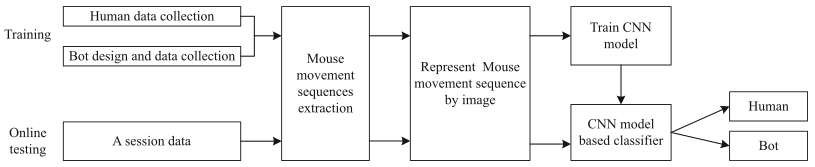
\includegraphics[width=1\columnwidth]{figures/deep_learning_with_mouse_dynamics_system_architecture}
    \caption{Architecture of the deep learning model using CNNs}
    {\small System design from~\cite{deep_learning_detection_with_mouse_behavior}}
    \label{fig:deep-learning-architecture}
\end{figure}
A user's botness is determined by considering the classification results of most mouse movement sequences extracted from the operation data created at the left-most, first stage of the architecture diagram.
Therefore, if the classifier depicts inputted mouose movement sequences to be that of a bot, than that particular user, or source of raw mouse position data, will be classified as a bot.
A few metrics were created to represent a user's mouse movement behavior:
\begin{itemize}
    \item \textbf{mouse movement sequence}: the records of a series of consecutive mouse moves
    \item \textbf{mouse trajectory}: a time-space curve corresponding to a mouse movement sequence
    \item \textbf{step size}: the distance between two consecutive points
    \item \textbf{event interval}: the time difference between two points
\end{itemize}
Similarly to this thesis research, the \textbf{mouse movement sequence}s are in the format $(x_i, y_i, t_i)$, where $i = 1{\dots}n$ with $n$ being the number of mouse positions in the sequence, $x$ and $y$ are the 2D coordinates of a mouse cursor's position, and $t$ is the time of when that cursor was at the respective position.

Representing a user's mouse movements is done by separating the continuous sequences of mouse events into segments of sequences that correspond to individual mouse movements.
Their assumption is that the intervals between mouse events does not exceed 100ms.
This closely aligns with the average mouse position polling rate of 125hz~\cite{mouse_dpi_and_polling_rate_explained}~\cite{mouse_dpi_and_usb_polling_rate}.
Any mouse movement sequence segments containing less that 15 events were discarded, as these events were said to not contain enough information for bot detection.
Following this sequence segmentation stage, a two-step process was implemented to transform the mouse movement sequence segments into images that can be used in the CNN model.

\textbf{Mapping spatial information into the image} was achieved by using shape and distance metrics between consecutive events of a segment.
The images were centered by finding the halfway point of the max distance between any two points in the segment.
Zoom was considered since the max distances vary among different segments.
With this in mind, all mouse positions in the segements were set to a constant 8px diameter.
\textbf{Mapping kinetic information into the image} was achieved by reflecting the event interval series and step size series.
The paper's denotations for these were $({\Delta}t_1,\dots,{\Delta}t_{n-1})$ and $({\Delta}d_1,\dots,{\Delta}d_{n-1})$ respectively.
In short, they used velocity as the feature to be represented in the images.
Every point in the segments were color-coded based on the magnitude of velocity calculated at each point.
The colors were on the red, blue, green (RGB) scale, and decided by mapping the delta values to an integer ranging from 0 to 255.
\begin{figure}[!h]
    \centering
    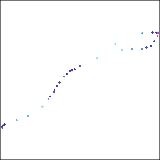
\includegraphics[width=.35\columnwidth]{figures/deep_learning_with_mouse_dynamics_mouse_segment_image_generation}
    \caption{Conversion of a mouse sequence segment to an image}
    \label{fig:deep-learning-image-generation}
    {\small Spatial and kinetic information of a users mouse movement behavior are represented in images similar to this one, as shown in~\cite{deep_learning_detection_with_mouse_behavior}. The mouse positions of mouse movement are shown in each sequence segment, a single image, and colors denote the velocity of mouse movement.}
\end{figure}
Bot users, specifically, were fabricated by 4 different types of bot scripts, each generating a unique pattern to their mouse movement trajectories.
Figure~\ref{fig:deep-learning-image-generation-bots} displays images that represent these 4 types.
\begin{figure}[!h]
    \centering
    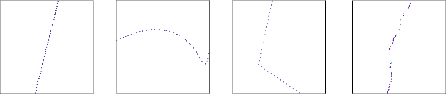
\includegraphics[width=1\columnwidth]{figures/deep_learning_with_mouse_dynamics_mouse_segment_image_generation_bots}
    \caption{Conversion of bot mouse sequence segments to an image}
    \label{fig:deep-learning-image-generation-bots}
    {\small Shown are examples of the 4 different types of bot mouse trajectories: \textit{straight-line}, \textit{curve}, \textit{polyline}, and \textit{semi-straight line}, respectively, as shown in~\cite{deep_learning_detection_with_mouse_behavior}}
\end{figure}
The semi-straight line was created by adding noise to the points on the straight-line mouse trajectory.
Bezier curves were used to make the curve and polyline trajectories.
All mouse sequence segments were created with a few different intervals between mouse events.
These intervals were added by either a set constant value, uniformly distributed values, or values with a Gaussian distribution.
Human datasets were gathered over a 2 month period of recording the activity of several human users.
With these datasets, images were generated in the manner previously described, thus allowing for a supervised learning, CNN model approach.
Although this paper reflects 90-99\% detection accuracy for all 4 types of bots, their results may reflect a testing bias.
Since the authors of this paper implemented the bot datasets, their methods of detecting said bots may cause testing biased to their own implementations, thus skewing results.

\subsection{Graphs and CNNs}\label{subsec:graphs-and-cnns}
BotGraph\cite{botgraph} is one which represented the sitemap, or order of page indexing, of a user with a nodes-and-edges graph.
Since these generated graphs are images that represent a number of metrics based on user behavior, not user identification, the research utilized CNNs to predict users types of either bot or human.
The BotGraph research concludes that this approach yields about a 95\% success rate in detecting bots.

This article begins by introducing key concepts mentioned by a company that specializes in web bot detection, ShieldSquare, the difference of identity-based and behavior-based bot detection.
The identify-based method utilizes client-side JavaScript to collect parameters like browser fingerprints; a collection of information about your browser type and version, as well as your operating system, active plugins, timezone, language, screen resolution and various other active settings~\cite{browser_fingerprinting}.
Whereas behavior-based methods utilize the number pages visited per session, the duration of time per page visit, and the number of page revisits, etc.
This research more closely resembles the behavior-based method but instead represents such metrics via a graph image which, according to the research, contains more unique features per user.
The paper continues by introducing a violator blacklist, biometric data validation like scroll and mouse movement method by Distil Networks, as well as the UserAgent variable present in HTTP protocol; an unstable bot-detection method as more advanced bots can falsify their identity by simply hiding or modifying the UserAgent variable.
DeepDefense~\cite{deep_defense_article} introduced a recurrent neural network (RNN)-based model that takes as input same-shape segment splits from the web server access logs, then encoded the request information in each line of segment to a numerical matrix.
The paper states that, while this method is most similar to the outlined research implementation, the inference efficiency of Deep Defense relies too heavily on the length of the same-shape segments; in which BotGraph supposedly proves to be more stable.

The research implementation included BotGraph, a program that generates graph-based representations of users' sitemap traversals.
Since these graphs were in image format, the implementation employed convolutional neural network (CNN) inferences to distinguish bots from human user types.
The details of BotGraph are as follows:
\begin{itemize}
    \item request - timestamp, HTTP method, request URI, status, host IP, user{\_}agent, client IP variables
    \item session - a method if identifying a series of client requests (by bot or human)
    \item identity - user{\_}agent and client IP variables for the client, and host IP variable for the server
    \item behavior - request URI and status variables for the access frequency metric per graph node.
\end{itemize}
The graph can be described as $G = (V, E)$:
\begin{itemize}
    \item $G$: a directed graph
    \item $V$: set of nodes representing all same-pattern URLs visited, i.e \textbf{/page?id=3} is pattern \textbf{/page?id=*}
    \item $E$: set of directed edges, each representing access points, i.e. \textbf{\textit{a}} tag elements with same href
\end{itemize}
Below is a figure of the BotGraph architecture. As you can see, BotGraph runs in a three-step process:
\begin{enumerate}
    \item Build a sitemap through one of three methods: \textit{active crawling, passive sniffing, self providing}
    \begin {enumerate}
        \item \textit{active crawling}: crawling typically starts from website homepage and recursively enters each hyperlink from the current page
        \item \textit{passive sniffing}: a website’s traffic is monitored, learned then used to build the sitemap. This is a less intrusive alternative to active crawling
        \item \textit{self providing}: the site provides its own sitemap for bot detection. This is the most accurate
    \end{enumerate}
    \item Map requests listed in server access logs to denote sessions as subgraphs in a sitemap
    \item Generate 2-dimensional trace images, translating a bot detection task into an image recognition
\end{enumerate}
\begin{figure}[!h]
    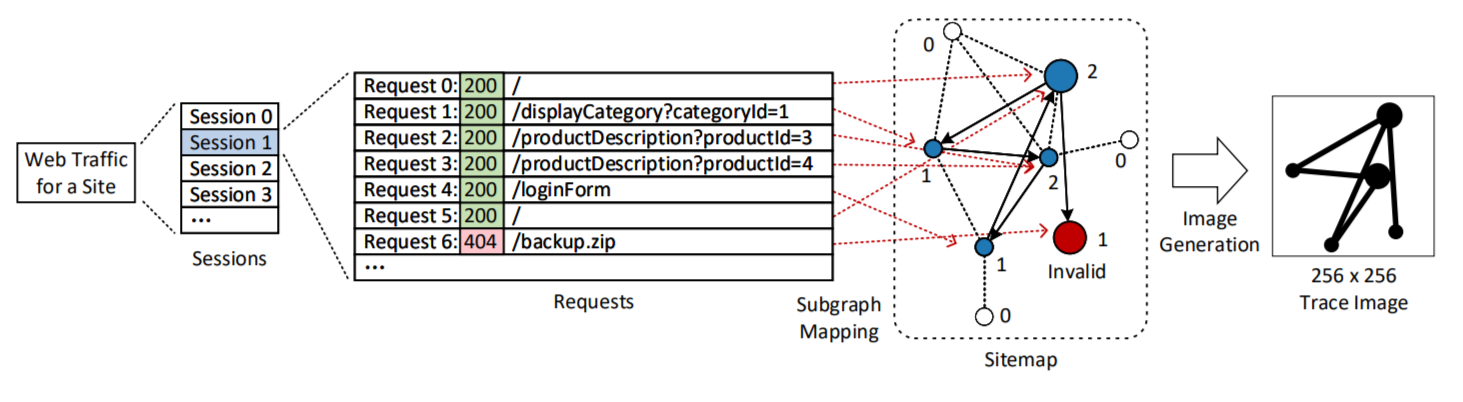
\includegraphics[width=1\columnwidth]{figures/BotGraph_fig1}
    \caption{Architecture of BotGraph}
    {\small Diagram from BotGraph~\cite{botgraph}}
    \label{fig:botgraph}
\end{figure}
This implementation used a model trained on a data set generated by 30+ professionals that manually tagged web traffic via JavaScript support checking, mouse movement and click tracking, IP reputation, UserAgent blacklisting.

A weakness in the BotGraph method of bot detection is when a user visits a lower number pages per session, i.e. less than 3 visits.
This is because bot and human users have too similar browsing behavior, namely their session sitemap traversal, creating near-identical sitemap graphs.
However, this research claims that BotGraph is a very effective and efficient method of detecting bots as it achieves about 95\% in precision and recall while relying only on the client's behavior and not the client's identity variables.
Some needed improvements include an implementation that generates more detailed graph-related features to better describe the characteristics of user sessions, specifically to identify the behavior of web bots.

\subsection{Training Data Generation and Semi-Supervised Learning}\label{subsec:training-data-generation-and-semi-supervised-learning}
The research described in~\cite{bot_detection_for_search_engines} addresses the common problem with supervised learning-based bot detection schemes.
Due to the high traffic of modern search engines, it is infeasible to rely on human judges to generate labeled datasets, used in supervised learning approaches, by manually inspecting the search logs to label bot and human users.
On a controlled webserver environment, labeled datasets were created by analyzing the response and activity of CAPTCHA challenges sent to the users.
In an effort to enhance the user experience, challenges were sent selectively, either when the webserver is experiencing a high volume of network traffic, or when a user makes a high number of requests in a short amount of time.
When presented with a challenge, the user can either disregard the challenge by exiting the session, answer correctly, or answer correctly, thus answering "no response", "correct response", or "wrong response", respectively.
\begin{figure}[!h]
    \centering
    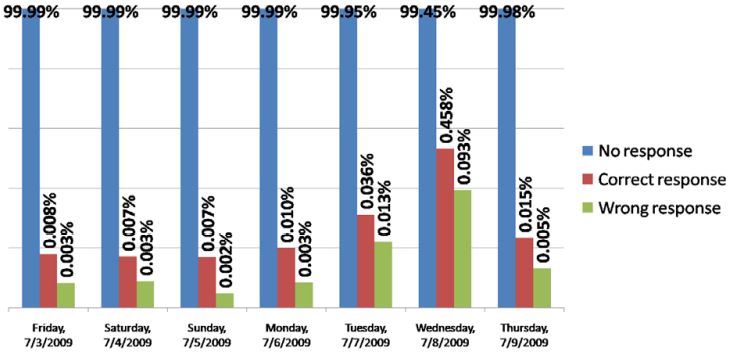
\includegraphics[width=1\columnwidth]{figures/semi_supervised_CAPTCHA_training_data_generation_results}
    \caption{User answers to CAPTCHA challenges}
    \label{fig:captcha-user-answers}
    {\small The research notes that since the users were selected non-uniformly, most answers to the challenge were "no response", as shown in~\cite{bot_detection_for_search_engines}}
\end{figure}
About 80\% of the received responses were correct.
This accounted for the majority of the training data with "human" labels.
The remaining "human" labels were pulled from the large set of "no response" answers by analyzing heuristics of the user's number of clicks in a time period, the number of search result pages browsed, as well as information of the user's IP address.
Users were labeled "bot" if the user's answer was "no response", and the user did not satisfy thresholds of the heuristics previously described.
This CAPTCHA challenge-method accounted for the "0-cost" training data generation method, as described in the research.

From the creation of the labeled training dataset, the following features were extracted from the users:
\begin{itemize}
    \item \textbf{PageTrackedCount}: measures the number of pages that the user browses
    \item \textbf{UserClickCount}: measures the number of mouse clicks on the search result pages
    \item \textbf{AllHitCount}: measures the overall "impressions" that the user receives in addition to the search results
    \item \textbf{UserUniqueIPs}: measures the unique number of IPs a user is using
    \item \textbf{UserUniqueQueries}: measures the unique number of queries issued by a single user in a search session
    \item \textbf{Blacklisting Rules}:
    \begin{enumerate}
        \item \textbf{Form}: triggered when a user includes in the query certain obscure codes that are designed mostly for internal search engine instrumentation purposes that should be unfamiliar to most genuine human users
        \item \textbf{IP}: a list of IPs that are publicly identified as Internet spammers and labeled all the traffic from these IPs as "bot"
        \item \textbf{Query}:  this rule is triggered when the query composition is too complicated to be manually typed in by a human user
    \end{enumerate}
\end{itemize}
The research stated, regarding the \textbf{PageTrackedCount}, that bots tend to behave in two extremes.
Some bots will only submit queries and not browse any of the result pages (except the first one), ostensibly with the intention to increase the query frequency for certain keywords.
The other extreme sees the bots fetch all the result pages for each query, probably trying to reverse engineer the index of the search engine, while genuine human users would probably just browse the first few pages of the query results selectively.
For \textbf{UserClickCount}, clicks on the search engine results, as well as clicks on advertisements within the results, were included in the click counts.
The research noted that the advertisement clicks, though are not distinguished in this work, may include bots specifically targeting ads to click.

With these features, a supervised learning method of bot detection was used.
In said research, the C4.5~\cite{c4.5} algorithm was the decision tree used in lieu of a custom implementation, stating "details of the decision tree algorithm are omitted here".
By leveraging the autonomously created labeled training dataset, sourced from CAPTCHA response and filtered by following the previously mentioned heuristics, the decision tree algorithm was projected to work well.
However, despite the positive projections, the results have shown to be inconsistent from the true data distribution, begging the question of the classification's integrity.
This may be a result of the training dataset generation stage, since the "bot" labels are subject to the heuristics determined by domain experts.
A useful approach to this dilemma was their statistical method of using numerous unlabeled data, due to uncertainties in the "0-cost" training data generation.
Despite the evaluated performance improvement from the tested supervised learning approach, some inconsistencies would need to be addressed in future work.
Due to the limited time of one week to present CAPTCHA challenges to users, some search engine bots may have been undetected, thus diminishing the integrity of the training data generation.
Therefore, it is unclear if this bot detection scheme can be as useful during more real, long-term scenarios.



\section{Decision Tree}\label{sec:decision-tree}

An implementation~\cite{bot_or_human} uses the C4.5 decision tree algorithm to determine if a user is a bot or not by characterizing human behaviors from bot behaviors in online services.
This approach consists of a two-step system that (1) extracts a user's behavioral metrics via a client-side logger, and (2) determines the botness of a user, based on the retrieved behavioral metrics, with a server-side classifier.
A client-side logger, in this context, records a user's behavioral metrics such as mouse movements and keystrokes.
Upon gathering this client-side data, the records are sent to the server-side classifier that utilizes the C4.5 decision tree algorithm.

There are two different bot detection approaches that this article seeks to address.
Firstly, \textbf{content-based filtering}, used by third party clients, needs to be improved upon since they suffer from high false negative rates.
This is due to mostly in part of the bot makers finding ways to evade filtering rules set by enforcers.
Secondly, \textbf{human interactive proofs} (HIPs), such as CAPTCHA, are problematic for more than one reason.
Not only are CAPTCHAs breakable by bot implementors, but the they are intrusive to the user experience.
Although there are ways to increase the reliability of HIPs to detect and block bots, such ways would require more interaction from the authentic human users, thus increasing user friction and diminishing the user experience.
Human observational proofs (HOBs) are a solution to this dilemma.
Unlike the HIPs that are commonly used, HOPs passively observe the actions and behavior of users performing tasks that are meant to be challenging for bots.

A blog site was the testing location for this research.
With over 65,000 users, averaging about 800 users simultaneously online, human user sessions were recorded to describe the various behavior characterizations.
Additionally, bot profiles were generated under 3 distinct categories (ranked by level of sophistication):
\begin{enumerate}
    \item \textbf{replay}: the most sophisticated type of bot, thus making it the most difficult bot to detect among the other 2 types.
        This bot records the actions of a human user doing something on the website, such as filling out a form or clicking on a button.
        Then the bot will impersonate that human user by replaying the recorded actions, exactly following the keystroke and mouse movement styles of that user.
    \item \textbf{mimic}: since most standard bot detection schemes use keystroke and mouse movement info, or the lackthereof, of the user to determine their botness, bot implementors need to include such details in their mimicking bot schemes.
        Using OS API calls to generate keystroke and mouse events, mimicking bots are able to bypass older or standard detection schemes.
        This is possible when a detection scheme only relies on UI events, such as mousemove, keystrokes, etc., which can be triggered by either hardware, such as a mouse and keyboard, or software, such as the OS API calls a mimicking bot would utilize.
    \item \textbf{inject}: while being the most common type of bot, this type of bot does not interact with the UI. Instead, it triggers the same code that UI events would tirgger, such as an HTTP request that would regularly be triggered by clicking on a UI button.
        Despite being detectable by most bot detection schemes, injection bots are still able to evade a server's check on HTTP protocols by forging certain fields in the headers, such as Referer, User Agent, and Cookie.
\end{enumerate}
While human user behavioral characterization data was collected from 1,078 signed-in site members during several two-hour monitoring sessions, bot user behavioral characterization data was collected by using existing libraries and frameworks.
For the injection bots, any UI features that triggered a POST request were instead triggered by cURL and a predifined string for the request body.
An open source Windows program, AutoHotkey, that is designed for automating the Windows GUI and for general scripting was used to configure the mimicking bot.
The AutoHotkey script they used was customized to the blog site, mimicking all sorts of human actions, such as moving, clicking, and scrolling the mouse cursor, as well as typing keys.
All mimicked actions were masked by entropies, such as random speeds of mouse movements or random delays when typing, to create some sort of human-like characteristics.
With the ability to record and replay mouse and keyboard API calls, the Global Mouse and Keyboard Library for Windows was used to configure the replay bot.

Their detection system design consists of a webpage-embeded logger, that records a user's behavior on the client-side, and a server-side classifier that considers the user's data from the client-side and determines if that user is a bot or not.
\begin{figure}[!h]
    \centering
    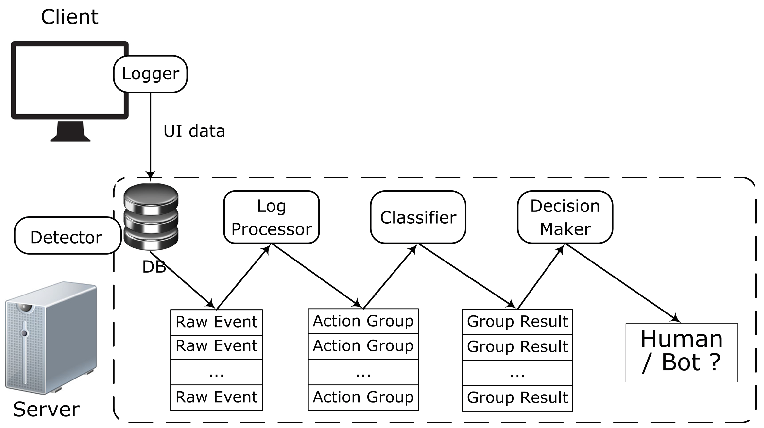
\includegraphics[width=.8\columnwidth]{figures/bot_or_human_system_architecture}
    \caption{Architecture of the client-side Logger and server-side Detector}
    \label{fig:bot-or-human-architecture}
\end{figure}
Similarly to this thesis research implementation, the client-side Logger is JavaScript code that stores UI event recordings into a buffer and periodically POSTs data to the server.
Mouse metrics are recorded at an average of 125hz polling rate.
Unbeknownst to the user, the Logger collects, via JavaScript events, five UI events: \textit{key press}, \textit{key release}, \textit{mouse move}, \textit{mouse button press}, and \textit{mouse button release}.
When the recordings are POSTed to the server-side Detector, a \textbf{log processor} begins to calculate the timing entropy of intervals of the whole raw event data sequence in the POSTed user log.
This detects periodic or regular timing of the entire user behavior.
Entropy rate can be used to distinguish a human user from a bot user.
Human behavior is often more complicated than bot behavior.
Such complexity can be measured by entropy rate.
Once the log processor finishes, the C4.5 algorithm is used as a base for the Detector's \textbf{classifier}.
Reasons for using the C4.5 decision tree algorithm include its efficiency to process large amounts of training data in a short time, the logic is easy to understand and not a black-box, the tree is able to process continuous and discrete values, and lastly, the tree has autonomous tree height constraints to avoid over fitting.
Finally, the \textbf{decision maker} in the Detector considers all classifications previously made on a user, and holistically makes a decision of its botness.



\section{Cluster Analysis}\label{sec:cluster-analysis}

\subsection{Deductions by Similarities}\label{subsec:deductions-by-similarities}
The bot detection implementation~\cite{bot_detection_wei_alvarez} uses traffic analysis, unsupervised machine learning, removal of duplicate flows, and similarity between malicious and benign traffic flows to provide insight on the botness of a web user.
The research refers to bot web traffic as malicious web traffic and non-malicious web traffic as benign web traffic, which may contain bots that are considered not harmful and are necessary to a system.
Search engine bots, for example, would be categorized as benign web traffic.
A series of clustering algorithms were tested and used to determine which clusters contained the most flows, leading to insight on the characteristics of a bot.
By conducting similarity analysis among these clusters, the work in this research provides a similarity coefficient to describe how malicious traffic data can be distinguished from benign traffic data.

Majority clusters were identified by the number of flows in a cluster.
Since the dataset contained mostly malicious flows, the cluster containing the most flows would also be the malicious flows cluster.
If this was not the case, than the clustering accuracy was therefore to be inaccurate.
Duplicate flows are flows that share the same values for the selected features, a set of networking-related metrics pertaining to packets traveling to and from the webserver.
Similarity between clusters was evaluated using the Jaccard Similarity Coefficient, which was a number ranging from 0 to 1 and the number was the cardinality of the intersection between two clusters, divided by the cardinality of the union between two clusters.

K-means was used to cluster benign and malicious flows, where k = 2.
Although the number of clusters was set known to be two, and the features in these clusters was not biometric data like mouse movement, the method of feature engineering was used as inspiration in this thesis work.
Removal of duplicate flows were shown to make the Jaccard Coefficient less computationally expensive.
However, a large reduction of duplicate flows within a cluster indicated that the cluster contained bots of a botnet.
Detecting anomalies such as this is important to consider when engineering features, a crucial step in the clustering process, in this thesis work.

\subsection{Outlier Detection}\label{subsec:outlier-detection}
There exists a few methods of outlier detection in bot and human user profiles.
Traditional \textbf{statistical outlier detection methods} are univariate.
Such techniques measure a particular atribute in a data distribution, while examining the degree of that value's outlierness.
The parameters, either known or unknown, the number of expected outliers, and the types of expected outliers are the focus of a statistical method.
Commons statistical measures, for example mean and standard deviation, can help find outliers in datasets.
For \textbf{density-based outlier detection methods}, the data points, and their relations to neighbors, are an integral metric to identifying outliers.
By definition, a datapoint is considered an outlier if there aren't many datapoints, or neighbors, near it.
One common algorithm, local outlier factor, measures the density of a datapoint withing a given k-number of datapoint pertaining to the nearest neighbors of a datapoint
Through this approach, outliers are identified as datapoints that have a substantially lower density that its neighbors.
A drawback to this approach, as well as other similar approaches, is that it's only capable of measuring the outlierness of a single datapoint, while it's incapable of identifying clusters of outliers.
Similarly, \textbf{distance-based outlier detection methods} is a method that may apply the local outlier factor.
A key benefit to the distance-based method is its ability to detect single datapoint outliers, as well as clusters of outliers.

The implementation~\cite{particle_swarm} uses outlier detection with a particle swarm optimization algorithm, hierarchical particle swarm based clustering, to detect web bots among human users.
Web bots are said to be examples of outliers since they are able to index a large number of pages in a short amount of time, contrary to human users.
There were two modules included in this work: a clustering module and an outlier detection module.
Both modules work simultaneously to label suspecting outliers, while the clustering module performs clustering in a hierarchical agglomerative manner.
Meanwhile, the outlier detection removes user profiles, that are labeled as suspecting outliers, from succeeding clusters.

This implementation was tested by using a dataset of user profiles that mimic a bots' behavior, as well as dataset without any ground truth, meaning the dataset contained user profiles without labels of their botness.
Three different metrics were used to predict the botness of user profiles: average intra-cluster distance, maximum intra-cluster distance, and the intersection of the average and maximum intra-cluster distances.
The results have shown that, by using the average and maximum intra-cluster distance metrics, bots are detectable when they are "significantly different from [a] legitimate web user" ~\cite{particle_swarm}.

Content goes here~\cite{optimized_outlier_bot_detection}



\chapter{System Design}\label{ch:system-design}


\section{Objective}\label{sec:objective}
The objective of this project is to present a novel approach for website administrators to detect web bots.
Supervised learning is a common ML approach to detect web bots.
In fact, most ML approaches to robot detection apply supervised learning~\cite{10.1145/3339252.3339267}.
This sort of approach consists of training a classifier, i.e.
a function mapping an input, which are usually feature vectors describing sessions, to an output, a session’s class labels, based on a training dataset, which includes labelled training samples.
The ability of the inferred function to determine correct class labels for new, unseen samples is assessed on a test dataset.
Many supervised learning techniques demonstrated their efficiency in classification of bots and humans, e.g., decision trees support vector machine, neural networks , and k-Nearest Neighbours.
All supervised learning approaches, however, share a common disadvantage, related to a difficulty with preparation of a reliable training dataset, in particular with assigning accurate class labels to sessions of camouflaged robots~\cite{ROVETTA2020102577}.
In conclusion, since web bots are increasing in sophistication, meaning they are behaving more like humans in terms of mouse and HTTP request behavior~\cite{10.1109/DSN.2013.6575366}~\cite{7371507}, obtaining accurate training data that represents such complex web bots has been an issue.
This, combined with the anonymity of proxies that scramble the IP addresses of web bots, has motivated this project.




\bigbreak
\bigbreak
\bigbreak
\bigbreak
\section{General Architecture}\label{sec:general-arcitecture}
The general architecture of this implementation is as follows:
\begin{enumerate}
    \item \textbf{data extraction}: The position metrics, timestamp and coordinates, of the user's mouse cursor are collected from the user's computer and sent to the server for analysis. The \textit{Dataset} section~\ref{sec:dataset} outlines this stage.
    \item \textbf{features generation}: From the inputted raw data recorded and sent from the user's machine, features that characterize the raw data, and the user's session pertaining to it, are generated. The \textit{Features Engineering} section~\ref{sec:features-engineering} outlines this stage.
    \item \textbf{clustering}: Sessions are clustered based on the generated features. The \textit{Clustering} section~\ref{sec:clustering} outlines this stage.
    \item \textbf{classification}: Clusters of sessions are used to determine bottness of users at client IP addresses. The \textit{Classification} section~\ref{sec:classification} outlines this stage, a stage anticipated for future work.
\end{enumerate}
\begin{figure}[!h]
    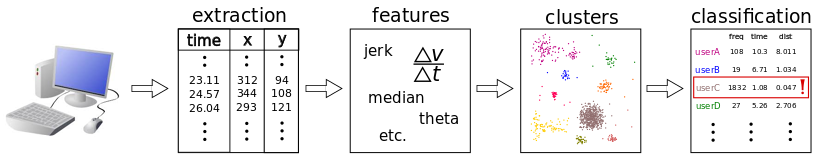
\includegraphics[width=1\columnwidth]{figures/general_architecture}
    \caption{Architecture of this bot detection scheme}
    \label{fig:general-architecture}
\end{figure}

The \textit{Implementation} chapter~\ref{ch:implementation} described how this architecture is built.



\chapter{Implementation}\label{ch:implementation}
This project will utilize an approach that begins by identifying users, which include human and bot users, based solely on their mouse movement behavior~\cite{intrustion_detection_using_mouse_dynamics}.
Specifically, this project presents a user differentiation method based on mouse behavior metrics, such as movement angle, movement velocity, scroll velocity, etc., instead of relying on client IP addresses present in the server logs.
Further study could include metrics that are also used in previously implemented web bot detection schemes.
But this project will start with just the mouse behavior metrics.
The presented approach in this project implies that, upon identifying users based on their mouse use behavior, decisions to declare userX, which is a single cluster, as a human or a bot are reinforced by empirical evidence of web traffic patterns corresponding to userX.
This approach could be an improvement to the inaccuracies present in previous supervised learning-based web bot detection schemes.
Additionally, this "identify users first, then classify as human or bot" method is similar to the current industry standard of websites requiring all visitors to log into an account for further use of their website; which reinforces decisions to declare account-holderX as a human or a bot, regardless of the IP address of account-holderX.
However, this "log-in, then use website" method causes user friction~\cite{how_recaptcha_is_improving_user_experience}, a concept introduced and considered by the latest "covert" versions of reCAPTCHA, that implies the inconveniences a user must experience to prove they are human and not a bot.
An example of this could be requiring a user to click/check "I'm not a robot" on older versions of reCAPTCHA.
In conclusion, this project presents an unsupervised, clustering method to autonomously identify users, as if they were to log in to an account, providing a means to make more informed decisions of the "web bot-ness" of visitors on a website.

\section{Objective}\label{sec:objective}
The objective of this project is to present a novel approach for website administrators to detect web bots.
Supervised learning is a common ML approach to detect web bots.
In fact, most ML approaches to robot detection apply supervised learning~\cite{10.1145/3339252.3339267}.
This sort of approach consists of training a classifier, i.e.
a function mapping an input, which are usually feature vectors describing sessions, to an output, a session’s class labels, based on a training dataset, which includes labelled training samples.
The ability of the inferred function to determine correct class labels for new, unseen samples is assessed on a test dataset.
Many supervised learning techniques demonstrated their efficiency in classification of bots and humans, e.g., decision trees support vector machine, neural networks , and k-Nearest Neighbours.
All supervised learning approaches, however, share a common disadvantage, related to a difficulty with preparation of a reliable training dataset, in particular with assigning accurate class labels to sessions of camouflaged robots~\cite{ROVETTA2020102577}.
In conclusion, since web bots are increasing in sophistication, meaning they are behaving more like humans in terms of mouse and HTTP request behavior~\cite{10.1109/DSN.2013.6575366}~\cite{7371507}, obtaining accurate training data that represents such complex web bots has been an issue.
This, combined with the anonymity of proxies that scramble the IP addresses of web bots, has motivated this project.

\section{General Architecture}\label{sec:general-arcitecture}
The general architecture of this implementation is as follows:
\begin{enumerate}
    \item \textbf{data extraction}: The position metrics, timestamp and coordinates, of the user's mouse cursor are collected from the user's computer and sent to the server for analysis. The \textit{Dataset} section outlines this stage.
    \item \textbf{features generation}: From the inputted raw data recorded and sent from the user's machine, features that characterize the raw data, and the user's session pertaining to it, are generated. The \textit{Features Engineering} section outlines this stage.
    \item \textbf{features analysis}: Sessions are clustered based on the generated features. The \textit{Features Analysis} section outlines this stage.
    \item \textbf{classification}: Clusters of sessions are used to determine bottness of users at client IP addresses. The \textit{Classification} section outlines this stage, a stage anticipated for future work.
\end{enumerate}
\begin{center}
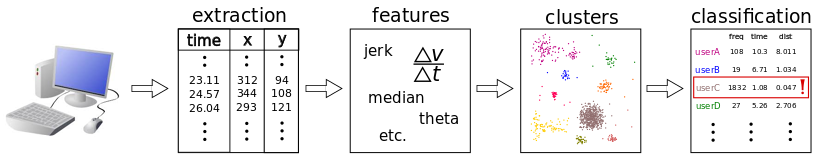
\includegraphics[width=1\columnwidth]{figures/general_architecture}
\end{center}

\section{Dataset}\label{sec:dataset}
In order to cluster users based on their mouse movement behavior, data of their mouse movement must be obtained.
An ideal scenario for this research would be to record the mouse movement of a high number of users, while navigating a specified user interface, thus creating a mouse movement recordings dataset.
But there are alternatives that maintain the validity of this research.

\subsection{Balabit Dataset}\label{subsec:balabit-dataset}
For testing and analysis purposes, a predefined dataset of users were used in this research.
The Balabit Mouse Challenge Dataset~\cite{balabit_dataset} was the primary dataset used in this research.
This dataset includes timing and positioning information of a web user's mouse pointer.
The authors of the dataset advertise that it can be used for authentication and identification purposes.
Researchers with focus on creating and evaluating the performance of behavioral biometric algorithms, which in this case draws from the mouse movement metrics of a user, are an intended audience for this publicly accessible dataset.
Originating from a data science competition on datapallet.io, the dataset is helpful to researchers and experts in the fields of IT security and datascience.

The competition for which the Balabit dataset originates from included a challenge of protecting users from unauthorized accesses into their accounts.
When users would login to their account, located on a remote server, recording their mouse movement behavior was a necessary step in an effort to increase account security.
Supposing that the method for which a user moves their mouse was unique to that user, a sort of biometric identifier can be obtained for account user authenticity.
If the mouse movement characteristics of a user, in a particular session, does not match the recorded and expected characteristics of the account holder, than that user in the particular session is said to be an unauthorized accessor.
In order to apply such a intrusion detection schema, a supervised learning-based model would need to be built and utilized.
However, this research does not intend on detecting unauthorized accessors, nor does it intend on using supervised learning in its implementation.

Although the Balabit dataset was intended to be used for creating and evaluating supervised learning-based models, the dataset still contains valuable user profiles and session recordings.
These user profiles are defined by a series of session recordings that are labeled with a single user of an account.
There are about 100 to 200 sessions recordings, spread over 10 users, with an average of 15 minutes of recording time per session.
Session recordings are split into two sets: training and testing.
This is for supervised learning uses.
For this research, all session files were combined into one set that is to be clustered and analyzed.
A session record is a csv file containing these fields~\cite{balabit_dataset}:
\begin{itemize}
    \item \textbf{record timestamp}: elapsed time (in seconds) since the start of the session as recorded by the network monitoring device used in the creation of the Balabit dataset
    \item \textbf{client timestamp}: elapsed time (in seconds) since the start of the session as recorded by the RDP client used by each of the 10 users
    \item \textbf{button}: the current condition of the mouse buttons
    \item \textbf{state}: additional information about the current state of the mouse
    \item \textbf{x}: the x coordinate (in pixels) of the mouse cursor on the screen
    \item \textbf{y}: the y coordinate (in pixels) of the mouse cursor on the screen
\end{itemize}
An example of a session record looks like:
\begin{center}
    \begin{tabular}{ |c|c|c|c|c|c| }
        \hline
        \textbf{record timestamp} & \textbf{client timestamp} & \textbf{button} & \textbf{state} & \textbf{x} & \textbf{y} \\
        \hline
        0.0 & 0.0 & NoButton & Move & 399 & 962 \\
        0.157999992371 & 0.155999999959 & NoButton & Move & 402 & 962 \\
        0.365999937057 & 0.248999999953 & NoButton & Move & 407 & 962 \\
        0.365999937057 & 0.358000000007 & Left & Pressed & 430 & 962 \\
        0.476999998093 & 0.467999999993 & Left & Released & 474 & 963 \\
        \ldots & \ldots & \ldots & \ldots & \ldots & \ldots \\
        \hline
    \end{tabular}
\end{center}
%duplicate session_0335985747

\subsection{Realtime Dataset}\label{subsec:realtime-dataset}
In a realtime environment, where the user differentiating algorithm is deployed, mouse movement data would come from the browser on the user's computer.
By using JavaScript's mousemove event listener, the coordinates of a user's mouse can be determined and recorded while a user is in session.
On average, a computers mouse position is polled 125 times per second~\cite{mouse_dpi_and_polling_rate_explained}~\cite{mouse_dpi_and_usb_polling_rate}.
This means that if a 10 second user session is recorded, there should be an average of 1,250 mouse position records of any single user browsing a website.
Records can be in a csv format:
\begin{itemize}
    \item \textbf{time}: elapsed time (in seconds) since the start of the session as recorded by the user's browser
    \item \textbf{x}: the x coordinate (in pixels) of the mouse cursor on the screen
    \item \textbf{y}: the y coordinate (in pixels) of the mouse cursor on the screen
\end{itemize}
A typical recorded session of a user's mouse movement metrics would look like:
\begin{center}
    \begin{tabular}{ |c|c|c| }
        \hline
        \textbf{time} & \textbf{x} & \textbf{y} \\
        \hline
        0.0 & 241 & 93 \\
        0.008121 & 278 & 77 \\
        0.015828 & 291 & 54 \\
        0.026942 & 302 & 48 \\
        0.037201 & 317 & 50 \\
        \ldots & \ldots & \ldots \\
        \hline
    \end{tabular}
\end{center}
These records can be stored on the user's computer, most likely in the browser via a JavaScript variable, then periodically sent to the server for which the website is hosted.
From this input, on the server, the web bot and botnet detection scheme will begin.
Pseudo code that generalizes the process of obtaining and sending a user's mouse movement metrics looks like:

{\color{darkgray} // the list of "times" "x" and "y" values POSTed to the server}
\newline
{\color{blue} \textbf{var}} records;

{\color{blue} \textbf{function}} flushRecords(bufSize)
\newline
\hspace*{25pt} {\color{darkgray} // reallocate "bufSize" number of indices for "times" "x" and "y" lists}

{\color{blue} \textbf{function}} postAndFlushRecords(bufSize)
\newline
\hspace*{25pt} {\color{darkgray} // POST all recorded "times" "x" and "y" values to the server}

{\color{blue} \textbf{function}} log(elapsedTime, x, y, bufSize)
\newline
\hspace*{25pt} {\color{darkgray} // insert "elapsedTime" "x" and "y" values into "records"}
\newline
\hspace*{25pt} {\color{darkgray} // postAndFlushRecords() if there are "bufSize" number of records}

{\color{blue} \textbf{function}} initBufferTimeout(timeLimit, bufSize)
\newline
\hspace*{25pt} {\color{darkgray} // postAndFlushRecords() every "timeLimit" duration}

{\color{blue} \textbf{function}} init()
\newline
\hspace*{25pt} {\color{darkgray} // use the "window" object's "onmousemove" func to log() mouse positions}
\newline
\hspace*{25pt} {\color{darkgray} // initBufferTimeout() to periodically POST logged "records" to the server}

{\color{darkgray} // called once upon every page load}
\newline
init();

The actual code, client{\_}mouse{\_}tracker.js, can be found in the src/ dir on the remote repo~\cite{thesis_github_repo} of this research.

\section{Features Engineering}\label{sec:features-engineering}
The intrustion detection scheme~\cite{intrustion_detection_using_mouse_dynamics}, while also using the Balabit dataset as it was intended to be used, extracted a set of features from the raw mouse position data.
Though their work implemented a supervised learning-based binary classifier, the features they extracted were proven to be effective metrics in differentiating and identifying users.
Instead of using all 6 elements of a datapoint vector, as outlined in the \textit{Balabit Dataset} section, we elected to only use the client timestamp ($t$), x position ($x$), and y position ($y$) values.
These three values construct a triplet, ($t_i$, $x_i$, $y_i$), $i = 1{\dots}n$, where $n$ is the number of recorded mouse positions, or datapoint vectors, in a session file.
From these three values, or triplets, of a single datapoint vector, in the list of vectors of a session file, the following features were extracted:
\begin{itemize}
    \item \textbf{velocity}: $v_i = \frac{\Delta d_i}{\Delta t_i}$
    \item \textbf{horizontal velocity}: ${v_x}_i = \frac{\Delta x_i}{\Delta t_i}$
    \item \textbf{vertical velocity}: ${v_y}_i = \frac{\Delta y_i}{\Delta t_i}$
    \item \textbf{acceleration}: $a_i = \frac{\Delta v_i}{\Delta t_i}$
    \item \textbf{jerk}: $j_i = \frac{\Delta a_i}{\Delta t_i}$
    \item \textbf{theta}: $\Theta _i = \arctan 2(\frac{\Delta y_i}{\Delta x_i})$
\end{itemize}

\subsection{Realtime Generation}\label{subsec:realtime-generation}
As described in the objective, this implementation is meant to detect web bots and botnet attacks in realtime.
At this stage of the detection scheme, a program would need to be run in realtime to compute the 6 features outline above.
Initially, a Python program was used to generate these 6 features as described.
The program calculated all 1676 session files, from all 10 users, in an average of 7 minutes.



\chapter{Evaluation}\label{ch:evaluation}


\section{Raw Data Extraction}\label{sec:evaluation-raw-data-extraction}



\section{Features Generation}\label{sec:evaluation-features-generation}



\section{Clustering}\label{sec:evaluation-clustering}



\section{Classification}\label{sec:evaluation-classification}




\nocite{*}
\bibliography{bibliography}

% Indents Appendix in Table of Contents
\makeatletter
\addtocontents{toc}{\let\protect\l@chapter\protect\l@section}
\makeatother

% Hack to make Appendices to appear in Table of Contents
\addtocontents{toc}{%
   \noindent APPENDICES
}
\begin{appendices}


\end{appendices}

\end{document}
